\documentclass[10pt,a4paper]{article}
\usepackage[margin=2cm]{geometry}
\usepackage[utf8]{inputenc}
\usepackage[T1]{fontenc}
\usepackage{listings}
\usepackage{enumitem}
\usepackage{color}
\usepackage{graphicx}
\usepackage{hyperref}
\usepackage{fourier}
\usepackage[scaled = 0.75]{beramono}
\usepackage{fancyhdr}
\usepackage{tikz}
\pagestyle{fancy}
\definecolor{myltgray}{rgb}{0.95,0.95,0.95}
\usepackage{textcomp}

\rhead{\raisebox{0.66ex}{\thepage}}
\lhead{\raisebox{0.66ex}{The Julia Express}\ \ 
\includegraphics[width=0.409cm]{rocketship11.png}}
\cfoot{}
\setlength\headheight{15pt}

\hypersetup{
    pdfstartview={FitH},
    pdftitle={Julia Express},
    pdfauthor={Bogumił Kamiński},
    colorlinks=true,
    linkcolor=blue,
    urlcolor=blue
}

\lstdefinelanguage{commentonly}{ morecomment=[l]{\#} }
\lstset{
  basicstyle=\ttfamily,
  backgroundcolor=\color{myltgray},
  commentstyle=\emph,
  language=commentonly,
  upquote=true
 }

\setlength{\parskip}{2pt}%
\setlength{\parindent}{0pt}

\begin{document}
\title{The Julia Express}
\author{Bogumił Kamiński}
\maketitle

{\centering

\includegraphics[width=0.2\textwidth]{rocketship11.png}\par
}

\tableofcontents

\section{Introduction}
The Purpose of this document is to introduce programmers to the Julia programming by example.
This is a simplified exposition of the language.\footnote{The rocket ship clip is free for download at \url{http://www.clipartlord.com/free-cartoon-rocketship-clip-art-2/}.}

It is simplest to execute these examples by copy-pasting to the Julia REPL (\url{https://docs.julialang.org/en/latest/stdlib/REPL/}) or copying them to a file and next running them using \lstinline|include| function. The difference is that copy-paste approach will echo output of each instruction to the terminal.

If some package is missing on your system switch to the package manager mode by pressing \lstinline|]| in the Julia REPL, and then write \lstinline|add [package name]| to require installing it.

This is an introductory document. Important topics that a person learning the Julia should be aware of, that are not covered are:
\begin{enumerate}[label=\arabic*),nolistsep]
  \item parametric types;
  \item parallel and distributed processing;
  \item advanced I/O operations;
  \item advanced package management;
  \item interaction with system shell; see \lstinline|run|;
  \item exception handling; see \lstinline|try|;
  \item creation of coroutines;
  \item integration with C, Fortran, Python and R.
\end{enumerate}
You can read about them in the latest Julia documentation at \url{http://julia.readthedocs.org/en/latest/manual/}.

\emph{The Julia Express} was tested using the following 64-bit Julia version:
\begin{lstlisting}
versioninfo()
# Julia Version 1.1.0
# Commit 80516ca202 (2019-01-21 21:24 UTC)
# Platform Info:
#   OS: Windows (x86_64-w64-mingw32)
#   CPU: Intel(R) Core(TM) i7-8550U CPU @ 1.80GHz
#   WORD_SIZE: 64
#   LIBM: libopenlibm
#   LLVM: libLLVM-6.0.1 (ORCJIT, skylake)
\end{lstlisting}

All suggestions how this guide can be improved are welcomed. Please contact me at \href{mailto:bkamins@sgh.waw.pl}{bkamins@sgh.waw.pl}.

\section{Getting around}

Running \lstinline|julia| invokes an interactive (REPL) mode. In this mode some useful commands are:
\begin{enumerate}[label=\arabic*),nolistsep]
  \item \lstinline|^D| (exits Julia);
  \item \lstinline|^C| (interrupts computations);
  \item \lstinline|?| (enters help mode);
  \item \lstinline|;| (enters system shell mode);
  \item \lstinline|]| (enters package manager mode);
  \item \lstinline|Ctrl-l| clears screen;
  \item putting \lstinline|;| after the expression will disable showing its value in REPL (not needed in scripts).
\end{enumerate}

Examples of some essential functions in the Julia REPL (they can be also invoked in scripts):
\begin{lstlisting}
  @edit max(1,2)      # show the definition of max function when invoked with arguments 1 and 2
  varinfo()           # list of global variables and their types
  cd("D:/")           # change working directory to D:/ (on Windows you can use /)
  pwd()               # get current working directory
  include("file.jl")  # execute source file
  exit(1)             # exit Julia with code 1 (exit code 0 is used by default)
  clipboard([1,2])    # copy data to system clipboard
  clipboard()         # load data from system clipboard as a string
\end{lstlisting}

You can execute a Julia script from OS shell by running \lstinline|julia script.jl|.

Try saving the following example script to a file and run it (more examples of all the constructs used are given in following sections):
\begin{lstlisting}
"""Sieve of Eratosthenes function docstring"""
function es(n::Int) # accepts one integer argument
    isprime = trues(n) # n-element vector of true-s
    isprime[1] = false # 1 is not a prime
    for i in 2:isqrt(n) # loop integers less or equal than sqrt(n)
        if isprime[i] # conditional evaluation
            for j in i^2:i:n # sequence with step i
                isprime[j] = false
            end
        end
    end
    return filter(x -> isprime[x], 1:n) # filter using an anonymous function
end

println(es(100))         # print all primes less or equal than 100
@time length(es(10^6))   # check function execution time and memory usage
\end{lstlisting}

\section{Basic literals and types}
Basic scalar literals are the following:
\begin{lstlisting}
  1::Int               # 64 bit integer on 64 bit Julia, no overflow warnings
  1.0::Float64         # 64 bit float, defines NaN, -Inf, Inf
  true::Bool           # boolean, allows "true" and "false"
  'c'::Char            # character, allows Unicode
  "s"::AbstractString  # strings, allows Unicode, see also Strings below
\end{lstlisting}
The syntax \lstinline|x::Type| is a literal \lstinline|x| with type \lstinline|Type| assertion. In practice the type assertion is not needed. Here we use it only to show the type of each kind of a literal. All basic types listed above are immutable.

Type assertions for variables are made in the same way and they can be useful to catch bugs in your code.

An important feature of integers in Julia is that by default they are 64 bit on 64 bit Julia and 32 bit on 32 bit Julia. This means that \lstinline|1::Int32| assertion will fail on 64-bit Julia. Notably \lstinline|Int| is a constant whose value is either \lstinline|Int64| or \lstinline|Int32| depending on version (the same with unsigned integer \lstinline|UInt|).

There is no automatic type conversion, unless some function explicitly performs it. This is especially important in function calls. The simplest way to perform the conversion of a value \lstinline|x| to type \lstinline|T| by writing \lstinline|T(x)|, for example:
\begin{lstlisting}
  Int64('a')     # character to integer
  Int64(2.0)     # float to integer
  Int64(1.3)     # inexact error
  Int64("a")     # error no conversion possible
  Float64(1)     # integer to float
  Bool(1)        # converts to boolean true
  Bool(0)        # converts to boolean false
  Bool(2)        # conversion error
  Char(89)       # integer to char
  string(true)   # cast Bool to string (works with other types, note small caps)
  string(1,true) # string can take more than one argument and concatenate them
  zero(10.0)     # zero of type of 10.0
  one(Int64)     # one of type Int64
\end{lstlisting}
General conversion can be done using \lstinline|convert(Type, x)| (typically \lstinline|convert| will not perform a copy if \lstinline|x| already has type \lstinline|Type|):
\begin{lstlisting}
  convert(Int64, 1.0) # convert float to integer
\end{lstlisting}
Parsing strings can be done using \lstinline|parse(Type, str)|:
\begin{lstlisting}
  parse(Int64, "1") # parse "1" string as Int64
\end{lstlisting}
Automatic promotion of many arguments to common type (if any exists) can be achieved using \lstinline|promote|:
\begin{lstlisting}
  promote(true, BigInt(1)//3, 1.0) # tuple (see Tuples) of BigFloats, true promoted to 1.0
  promote("a", 1)                  # promotion to a common type is not possible
\end{lstlisting}
Many operations (arithmetic, assignment) are defined in a way that performs automatic type promotion (so this is a way to work around no automatic type conversion rule in Julia).

One can verify type of a value in the following way:
\begin{lstlisting}
  typeof("abc")              # String returned which is a AbstractString subtype
  isa("abc", AbstractString) # true
  isa(1, Float64)            # false, integer is not a float
  isa(1.0, Float64)          # true
  1.0 isa Number             # an alternative syntax; true, Number is abstract type
  supertype(Int64)           # supertype of Int64
  subtypes(Real)             # subtypes of abstract type Real
\end{lstlisting}
It is possible to perform calculations using arbitrary precision arithmetic, complex and rational numbers:
\begin{lstlisting}
  BigInt(10)^1000   # big integer
  BigFloat(10)^1000 # big float, see documentation how to change default precision
  big(1.5)          # value of big type chosen appropriately, in this case BigFloat
  1 + 1im           # a complex number
  123//456          # rational numbers are created using // operator
\end{lstlisting}

\begin{figure}
\centering
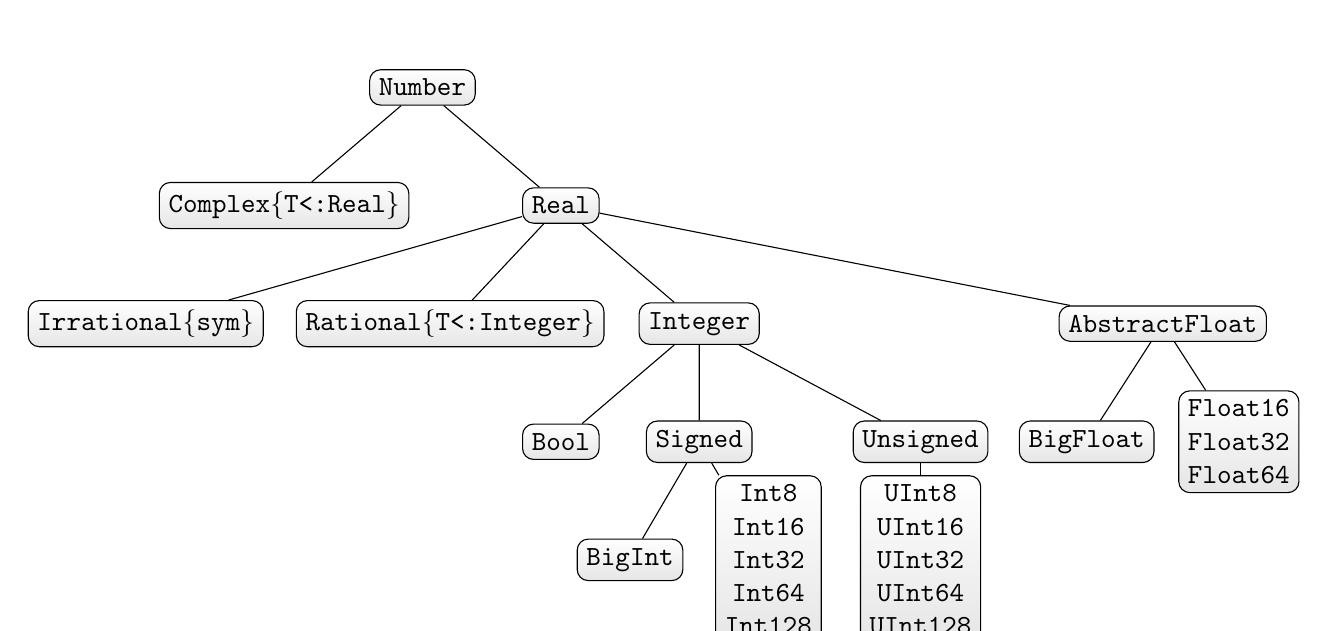
\begin{tikzpicture}[sibling distance=10em,
  every node/.style = {shape=rectangle, rounded corners,
    draw, align=center, font=\ttfamily,
    top color=white, bottom color=gray!20}]]
  \node {Number}
    child { node {Complex\{T<:Real\}} }
    child { node {Real}
        child { node {Irrational\{sym\}}}
        child[sibling distance=8em]{ node {Rational\{T<:Integer\}}}
        child { node {Integer}
            child[sibling distance=5em]{ node {Bool} }
            child[sibling distance=5em]{ node {Signed}
                child { node {BigInt} }
                child { node {Int8 \\ Int16 \\ Int32 \\ Int64 \\ Int128} }
            }
            child[sibling distance=8em]{ node {Unsigned}
                child { node {UInt8 \\ UInt16 \\ UInt32 \\ UInt64 \\ UInt128} }
            }
        }
        child[sibling distance=14.5em]{ node {AbstractFloat}
            child[sibling distance=5.5em]{ node {BigFloat} }
            child[sibling distance=5.5em]{ node {Float16 \\ Float32 \\ Float64} }
        }
    };
\end{tikzpicture}
\caption{Hierarchy of numeric types\label{fig:numeric}}
\end{figure}

Type hierarchy of all standard numeric types is given in Figure \ref{fig:numeric}.

\section{Special literals and types}
\begin{lstlisting}
  Any     # all objects are of this type
  Union{} # subtype of all types, no object can have this type
  Nothing # type indicating nothing (absence of a value), a subtype of Any
  nothing # only instance of Nothing
  Missing # type indicating missing value (a value exists but is unknown), a subtype of Any
  missing # only instance of Missing
\end{lstlisting}
Additionally \verb|#undef| indicates an incompletely initialized object element (see documentation for details).

\subsection{Tuples and NamedTuples}
Tuples are immutable sequences indexed from 1:
\begin{lstlisting}
  ()            # an empty tuple
  (1,)          # a one element tuple
  ("a", 1)      # a two element tuple
  ('a', false)::Tuple{Char, Bool} # tuple type assertion
  x = (1, 2, 3)
  x[1]          # 1 (element)
  x[1:2]        # (1, 2) (tuple)
  x[4]          # bounds error
  x[1] = 1      # error - a tuple is not mutable
  a, b = x      # tuple unpacking a==1, b==2
\end{lstlisting}
Additionally you can add names to tuple entries (via named tuples):
\begin{lstlisting}
  NamedTuple()  # an empty named tuple
  (a=1,)        # a one element named tuple
  (x="a", y=1)  # a two element named tuple
  x = (p=1, q=2, r=3)
  x.p           # access to element p of a tuple
  typeof(x)     # NamedTuple{(:p, :q, :r),Tuple{Int64,Int64,Int64}}, field names are part of type
\end{lstlisting}
Named tuple can be thought of as an anonymous \lstinline|struct| --- see composite types below (so they behave in a different way than tuples when testing for subtyping. This is an advanced topic that we do not cover in this introduction, see the Julia manual for the details \url{https://docs.julialang.org/en/latest/manual/types/}).

\subsection{Arrays}
Arrays are mutable and passed by reference.

Useful array creation functions are the following:
\begin{lstlisting}
  Array{Char}(undef, 2, 3, 4) # uninitialized 2x3x4 array of Chars
  Array{Int64}(undef, 0, 0)   # degenerate 0x0 array of Int64
  zeros(5)             # vector of Float64 zeros
  ones(5)              # vector of Float64 ones
  ones(Int64, 2, 1)    # 2x1 array of Int64 ones
  trues(3), falses(3)  # a tuple of a vector of trues and a vector of falses
  Matrix(I, 3, 3)      # 3x3 Bool identity matrix, requires to run first: using LinearAlgebra
  x = range(0, stop=1, length=11) # an iterator having 11 equally spaced elements
  collect(x)           # converts an iterator to vector
  1:10                 # iterable from 1 to 10
  1:2:10               # iterable from 1 to 9 with 2 skip
  reshape(1:12, 3, 4)  # a 3x4 matrix like object filled columnwise with values from 1 to 12
  fill("a", 2, 2)      # a 2x2 array filled with "a"
  repeat(rand(2,2), 3, 2) # a 2x2 random matrix repeated 3x2 times
  x = [1, 2]           # a two element vector
  resize!(x, 5)        # resize x in place to hold 5 values (filled with garbage)
  [1]                  # a vector with one element (not a scalar)
  [x * y for x in 1:2, y in 1:3] # a comprehension generating 2x3 array
  Float64[x^2 for x in 1:4] # casting comprehension result element type to Float64
  [1 2]                # 1x2 matrix (hcat function)
  [1 2]'               # 2x1 Adjoint matrix (reuses memory)
  permutedims([1 2])   # 2x1 matrix (permuted dimensions, new memory)
  [1, 2]               # vector (concatenation)
  [1; 2]               # vector (vcat function)
  [1 2 3; 1 2 3]       # 2x3 matrix (hvcat function)
  [1; 2] == [1 2]'     # false, different array dimensions
  hcat(1:2)==[1 2]'    # true, dimensions match
  [(1, 2)]             # 1-element vector
  collect((1, 2))      # 2-element vector by tuple unpacking
  [[1 2] 3]            # concatenate along rows (hcat)
  [[1; 2]; 3]          # concatenate along columns (vcat)
  tuple([1,2,3])       # a 1-element tuple containing a vector
  Tuple([1,2,3])       # a 3-element tuple unpacking a vector
\end{lstlisting}
Vectors (1D arrays) are treated as column vectors.

Most of the functionality for working with matrices are in \lstinline|LinearAlgebra| package.
Additionally Julia offers sparse and distributed matrices (see the documentation for details).

Commonly needed array utility functions:
\begin{lstlisting}
  a = [x * y for x in 1:2, y in 1, z in 1:3] # 2x3 array of Int64; a singleton dimension is dropped
  a = [x * y for x in 1:2, y in 1:1, z in 1:3] # 2x1x3 array of Int64; a singleton dimension is not dropped
  ndims(a)             # number of dimensions in a
  eltype(a)            # type of elements in a
  length(a)            # number of elements in a
  size(a)              # a tuple containing dimension sizes of a
  axes(a)              # a tuple of ranges specifying array axes
  eachindex(a)         # each index to an array a
  CartesianIndices(a)  # a lazy iterator over Cartesian indices into a
  LinearIndices(a)     # a lazy iterator over linear indices into a
  vec(a)               # cast an array to vector (single dimension)
  dropdims(a, dims=2)  # remove the 2nd dimension as it has length 1
  sum(a, dims=3)       # calculate sums for 3rd dimensions, similarly: mean, std,
                       # prod, minimum, maximum, any, all
  count(x -> x > 0, a) # count number of times a predicate is true, similar: all, any
\end{lstlisting}

Access functions:
\begin{lstlisting}
  a = 0:0.01:1         # range with step 0.01
  a[1]                 # get scalar 0.0
  a[end]               # get scalar 1.0 (last position)
  a[1:2:end]           # every second element from range
  view(a, 1:2:101)     # a view into a (a subarray of a)
  a[[1, 3, 6]]         # 1st, 3rd and 6th element of a, Array{Float64,1}
  lastindex(a)         # last index of the collection a; similarly firstindex
\end{lstlisting}

Observe the treatment of singleton dimensions:
\begin{lstlisting}
  a = reshape(1:12, 3, 4)
  a[:, 1:2]          # 3x2 matrix
  a[:, 1]            # 3 element vector
  a[1, :]            # 4 element vector
  a[1:1, :]          # 1x4 matrix
  a[:, :, 1, 1]      # works 3x4 matrix
  a[:, :, :, [true]] # works 3x4x1x1 matrix
  a[1, 1, [false]]   # works 0-element Array{Int64,1}
\end{lstlisting}

Array assignment:
\begin{lstlisting}
  x = collect(reshape(1:8, 2, 4))
  x[:,2:3] = [1 2]            # error; size mismatch
  x[:,2:3] .= [1 2]           # OK, broadcasting with .
  x[:,2:3] = repeat([1 2], 2) # OK
  x[:,2:3] .= 3               # OK, need to use broadcast with .
\end{lstlisting}

Arrays are assigned and passed by reference. Therefore copying is provided:
\begin{lstlisting}
  x = Array{Any}(undef, 2)
  x[1] = ones(2)
  x[2] = trues(3)
  a = x
  b = copy(x)     # shallow copy
  c = deepcopy(x) # deep copy
  x[1] = "Bang"
  x[2][1] = false
  a               # identical as x
  b               # only x[2][1] changed from the original x
  c               # contents of the original x
\end{lstlisting}

Array types syntax examples:
\begin{lstlisting}
  [1 2]::Array{Int64, 2}      # 2 dimensional array of Int64
  [true; false]::Vector{Bool} # vector of Bool
  [1 2; 3 4]::Matrix{Int64}   # matrix of Int64
\end{lstlisting}

Numbers are treated as 0-dimensional containers:
\begin{lstlisting}
  x = 10   # an integer
  x[]      # returns 10
  x[1,1]   # also returns 10, as trailing 1-s are ignored by Julia
  size(x)  # an empty tuple
  x = [10] # a one element array can be also indexed with []
  x[]      # gets you 10, this will only work for arrays with exactly 1 element
\end{lstlisting}

\subsection{Composite types}
You can define and access composite types. Here is an example of a mutable composite type:
\begin{lstlisting}
  mutable struct Point
    x::Int64
    y::Float64
    meta
  end
  p = Point(0, 0.0, "Origin")
  p.x               # access field
  p.meta = 2        # change field value
  p.x = 1.5         # error, wrong data type
  p.z = 1           # error - no such field
  fieldnames(Point) # get names of type fields
\end{lstlisting}

Similarly you can define some type to be immutable by removing \lstinline|mutable| keyword (named tuples are anonymous immutable structs).

There are also union types (see documentation of \emph{Type Unions} in the Julia manual for details).

Finally you can define that your type is a subtype of an abstract type to properly position it in the type hierarchy, or even define your own abstract types (see documentation of \emph{Abstract Types} in the Julia manual for details).

\subsection{Dictionaries}
Associative collections (key-value dictionaries):
\begin{lstlisting}
  x = Dict{Float64, Int64}()        # an empty dictionary mapping floats to integers
  y = Dict("a"=>1, "b"=>2)          # a filled dictionary
  y["a"]                            # element retrieval
  y["c"]                            # error
  y["c"] = 3                        # added element
  haskey(y, "b")                    # check if y contains key "b"
  keys(y), values(y)                # tuple of collections returning keys and values in y
  delete!(y, "b")                   # delete a key from a collection, see also: pop!
  get(y,"c","default")              # return y["c"] or "default" if not haskey(y,"c")
\end{lstlisting}
Julia also supports operations on sets, created similarly with \lstinline|Set| constructor (please refer to the documentation for details).

\section{Strings}
String operations:
\begin{lstlisting}
  "Hi " * "there!"       # string concatenation
  "Ho " ^ 3              # repeat string
  string("a = ", 123.3)  # create using print function
  repr(123.3)            # fetch value of show function to a string
  occursin("CD", "ABCD") # check if first string contains second
  "\"\n\t\$"             # C-like escaping in strings, new \$ escape
  x = 123
  "$x + 3 = $(x+3)"      # unescaped $ is used for interpolation
  "\$199"                # to get a $ symbol you must escape it
  raw"D:\path"           # a raw string literal; useful for paths under Windows
  s = "abc"              # a string of type String
  chop(s)                # remove last character from s, returns a SubString
\end{lstlisting}

Both \lstinline|String| and \lstinline|SubString| are subtypes of \lstinline|AbstractString|.
The  \lstinline|SubString| type is used to avoid copying of strings. Usually, when writing your own code,
it is best to assume that the user will pass an arbitrary \lstinline|AbstractString|.

PCRE regular expressions handling:
\begin{lstlisting}
  r = r"A|B"           # create new regexp
  occursin(r, "CD")    # false, no match found
  m = match(r, "ACBD") # find first regexp match, see the documentation for details
\end{lstlisting}

There is a vast number of string functions --- please refer to the documentation.

Warning! Note that you can index-into a string, e.g. \lstinline|"abc"[1]| will return you a character \lstinline|'a'|. However, in general Julia encodes standard strings using UTF-8 and indexing is based on bytes not characters, so correct string indexing requires you to understand how UTF-8 encoding works. See the documentation for details.

\section{Programming constructs}
The simplest way to bind a value to a new variable is by an assignment:
\begin{lstlisting}
  x = 1.0          # x is bound to Float64 value
  x = 1            # now x is bound to value Int32 on 32 bit machine and Int64 on 64 bit machine
\end{lstlisting}

Expressions can be compound using \lstinline|;| or \lstinline|begin end| block:
\begin{lstlisting}
  x = (a = 1; 2 * a) # after: x = 2; a = 1
  y = begin
    b = 3
    3 * b
  end              # after: y = 9; b = 3
\end{lstlisting}

There are standard programming constructs:
\begin{lstlisting}
  if false    # if clause requires Bool test
      z = 1
  elseif 1 == 2
      z = 2
  else
      a = 3
  end         # after this a = 3 and z is undefined

  1==2 ? "A" : "B" # standard ternary operator

  i = 1
  while true
      global i += 1 # global would not be needed if the loop were inside a function
      if i > 10
        break
      end
  end

  for x in 1:10    # x in collection, can also use = here instead of in
      if 3 < x < 6
          continue # skip one iteration
      end
      println(x)
  end              # x is defined in the inner scope of the loop
\end{lstlisting}

You can define your own functions:
\begin{lstlisting}
  f(x, y = 10) = x + y           # one line definition of a new function f with y defaulting to 10
                                 # last expression result returned
  function f(x, y=10)            # the same as above but allowing multiple expressions
      x + y                      # in the body of the function
  end
  f(3, 2)                        # a simple call, 5 returned
  f(3)                           # 13 returned
  (x -> x^2)(3)                  # an anonymous function with a call example
  () -> 0                        # an anonymous function with no arguments
  h(x...) = sum(x)/length(x) - mean(x) # a vararg function; x is a tuple
  h(1, 2, 3)                     # the result is 0
  x = (2, 3)                     # a tuple
  f(x)                           # error
  f(x...)                        # OK - tuple unpacking
  s(x; a = 1, b = 1) = x * a / b # function with keyword arguments a and b
  s(3, b = 2)                    # call with a keyword argument
  q(f::Function, x) = 2 * f(x)   # a function can be passed around; here we require that f is a Function
  q(x -> 2x, 10)                 # 40 returned, no need to use * in 2x (means 2*x)
  q(10) do x                     # creation of an anonymous function by do construct, useful eg. in IO
    2 * x
  end
  m = reshape(1:12, 3, 4)
  map(x -> x ^ 2, m)             # 3x4 array returned with transformed data
  filter(x -> bitstring(x)[end] == '0', 1:12)  # a fancy way to choose even integers from the range
  ==(1)                          # returns a function that tests for equality to 1
  findall(==(1), 1:10)           # find indices of all elements equal to 1, similar: findfirst, findlast
\end{lstlisting}

As a convention functions with name ending with \lstinline|!| change their arguments in-place. See for example \lstinline|resize!| in this document.

Default function arguments are evaluated left to right:
\begin{lstlisting}
  y = 10
  f1(x=y) = x; f1()      # 10
  f2(x=y,y=1) = x; f2()  # 10
  f3(y=1,x=y) = x; f3()  # 1
  f4(;x=y) = x; f4()     # 10
  f5(;x=y,y=1) = x; f5() # 10
  f6(;y=1,x=y) = x; f6() # 1
\end{lstlisting}

There is an important part of Julia terminology is that a \emph{function} can have multiple \emph{methods}. Each method specifies a behavior of a function for a given set of argument types. This behavior is called multiple dispatch and works only for positional arguments. Here are some short examples. More details are given in \emph{Methods} section of the Julia manual.
\begin{lstlisting}
  g(x, y) = println("all accepted") # method for g function accepting any type of x and y
  function g(x::Int, y::Int)        # method called when both x and y are Int
    y, x
  end
  g(x::Int, y::Bool) = x * y        # this will be called when x is Int and y is Bool
  g(1.0, 1)                         # the first definition is invoked
  g(1, 1)                           # the second definition is invoked
  g(1, true)                        # the third definition is invoked
  methods(g)                        # list all methods defined for g
  t(; x::Int64 = 2) = x             # a single keyword argument
  t()                               # 2 returned
  t(; x::Bool = true) = x           # no multiple dispatch for keyword arguments; function overwritten
  t()                               # true; old function was overwritten
\end{lstlisting}

\section{Variable scoping}
The following constructs introduce a new variable scope:
\lstinline|function|, \lstinline|while|,
\lstinline|for|, \lstinline|try/catch|,
\lstinline|let|, \lstinline|struct|, \lstinline|mutable struct|.

You can define variables as:
\begin{itemize}
  \item \lstinline|global|: use variable from a global scope of the current module;
  \item \lstinline|local|: define a new variable in a current scope;
  \item \lstinline|const|: ensure variable type is constant (global only).
\end{itemize}

Special cases:
\begin{lstlisting}
  t                  # error, a variable t does not exist
  f() = global t = 1
  f()                # after the call t is defined globally

  function f1(n)
    x = 0
    for i = 1:n
      x = i
    end
    x
  end
  f1(10)            # 10; inside the loop we use the outer local variable

  function f2(n)
    x = 0
    for i = 1:n
      local x
      x = i
    end
    x
  end
  f2(10)            # 0; inside loop we use new local variable

  function f3(n)
    for i = 1:n
      h = i
    end
    h
  end
  f3(10)            # error; h not defined in outer scope

  const x = 2
  x = 3 # warning, value changed
  x = 3.0 # error, wrong type

  function f()
      x::Int = 1
      x = 2.5 # error will be thrown when f() is called as x has to have type Int
  end
\end{lstlisting}
Global constants speed up code execution as the compiler knows their type.

Loops and comprehensions rebind variables on each iteration, so they are safe to use then creating closures in iteration:
\begin{lstlisting}
  Fs = Array{Any}(undef, 2)
  for i in 1:2
    Fs[i] = () -> i
  end
  Fs[1](), Fs[2]() # (1, 2)
\end{lstlisting}

\section{Modules}
Modules encapsulate code and each module has its own global name space (module name of Julia REPL is \lstinline|Main|).
\begin{lstlisting}
  module M # module name
  export x # what module exposes for the world
  x = 1
  y = 2 # hidden variable
  end

  varinfo(M) # list exported variables
  x       # not found in global scope
  M.y     # direct variable access possible

  # import all exported variables
  # also load standard packages this way, but without . prefix
  using .M

  #import variable y to global scope (even if not exported)
  import .M.y
\end{lstlisting}
Rebinding values of variables defined in other modules is not allowed. Here is a short typical example that often surprises people:
\begin{lstlisting}
  sin(1) # works
  sin = 1 # fails in module Main you cannot rebind a value defined in module Base
  cos = 1 # works, as cos was not called yet so it was not imported from Base into Main
  cos # returns 1
  cos(1) # fails - cos is bound to 1 in the module Main
  Base.cos(1) # works
\end{lstlisting}

\section{Operators}
Julia follows standard operators with the following quirks:
\begin{lstlisting}
  true || false    # binary or operator (singletons only), || and && use short-circut evaluation
  [1 2] .& [2 1]   # bitwise and operator (vectorized by .)
  1 < 2 < 3        # chaining conditions is OK (singletons only without .)
  [1 2] .< [2 1]   # for vectorized operators need to add '.' in front
  x = [1 2 3]
  2x + 2(x .+ 1)   # multiplication can be omitted between a literal and a variable or a left parenthesis
  y = [1, 2, 3]
  x + y  # an error
  x .+ y # a 3x3 matrix, dimension broadcasting
  x + y' # a 1x3 matrix
  x * y  # array multiplication, a 1-element vector (not scalar)
  x .* y # element-wise multiplication, a 3x3 array

  x == [1 2 3]  # true, object looks the same
  x === [1 2 3] # false, objects not identical

  z = reshape(1:9, 3, 3)
  z + x  # error
  z .+ x # x broadcasted vertically
  z .+ y # y broadcasted horizontally

  # an explicit broadcast of singleton dimensions
  # function + is called for each array element
  broadcast(+, [1 2], [1; 2])
  # broadcasting using . operator
  using Random
  length([randstring(10) for i in 1:5]) # 5 - length of an array
  length.([randstring(10) for i in 1:5]) # 5-element array of 10s - lengths of strings
\end{lstlisting}

Function broadcasting examples:
\begin{lstlisting}
  t(x::Float64, y::Float64 = 1.0) = x * y
  t(1.0, 2.0)               # OK
  t([1.0 2.0])              # error
  t.([1.0 2.0])             # OK
  t([1.0 2.0], 2.0)         # error
  t.([1.0 2.0], 2.0)        # OK
  t.(2.0, [1.0 2.0])        # OK
  t.([1.0 2.0], [1.0 2.0])  # OK
  t.([1.0, 2.0], [1.0 2.0]) # OK
\end{lstlisting}

\section{Essential general usage functions}
\begin{lstlisting}
  show(collect(1:100)) # show text representation of an object
  eps()             # distance from 1.0 to next representable Float64
  nextfloat(2.0)    # next float representable, similarly provided prevfloat
  isequal(NaN, NaN) # true
  NaN == NaN        # false
  NaN === NaN       # true
  isequal(1, 1.0)   # true
  1 == 1.0          # true
  1 === 1.0         # false
  0.0 == -0.0       # true
  0.0 === -0.0      # false
  isfinite(Inf)     # false, similarly provided: isinf, isnan
  fld(-5, 3), mod(-5, 3) # (-2, 1), division towards minus infinity
  div(-5, 3), rem(-5, 3) # (-1, -2), division towards zero
  findall(x -> mod(x, 2) == 0, 1:8) # find indices for which function returns true
  x = [1 2]; identity(x) === x # true, identity function
  @info "Info"      # print information, similarly @warn and @error (see Logging module)
  ntuple(x->2x, 3)  # create tuple by calling x->2x with values 1, 2 and 3
  @isdefined x      # if variable x is defined
  y = Array{Any}(undef,2); isassigned(y, 3)  # if position 3 in array is assigned (not out of bounds or #undef)
  fieldtype(typeof(1:2),:start) # get type of the field in composite type (passed as symbol)
  fieldnames(typeof(1:2)) # get field names of a type
  zip(1:3, 1:3) |> collect # convert iterables to iterable tuple and pass it to collect
  enumerate("abc")  # create iterator of tuples (index, collection element)
  collect(enumerate("abc")) # and materialize it
  isempty("abc")    # check if a collection is empty; strings are treated as collections of characters
  'b' in "abc"      # check if element is in a collection
  indexin(collect("abc"), collect("abrakadabra")) # [1, 2, nothing] ('c' not found), needs arrays
  findall(in("abrakadabra"), "abc") # [1, 2] ('c' was not found)
  unique("abrakadabra") # return unique elements
  issubset("abc", "abcd") # check if every element in fist collection is in the second
  argmax("abrakadabra") # an index of maximal element (3 - 'r' in this case)
  findmax("abrakadabra") # tuple: a maximal element and its index
  filter(x->mod(x,2)==0, 1:10) # retain elements of a collection that meet predicate
  dump(1:2:5)       # show all user-visible structure of an object
  sort(rand(10))    # sort 10 uniform random values, sort! for in-place operation
\end{lstlisting}

\section{Reading and writing data}
For I/O details refer documentation. There are numerous packages providing this functionality.
Basic operations from \lstinline|DelimitedFiles| package:
\begin{itemize}
  \item \lstinline|readdlm|: read from file
  \item \lstinline|writedlm|: write to a file
\end{itemize}

Warning! Trailing spaces are not discarded if \lstinline|delim=' '| in file reading.

\section{Random numbers}
Basic random numbers:
\begin{lstlisting}
  Random.seed!(1) # set random number generator seed to 1; needs calling first: using Random
  rand()        # generate random number from U[0,1)
  rand(3, 4)    # generate 3x4 matrix of random numbers from U[0,1]
  rand(2:5, 10) # generate vector of 10 random integer numbers in range form 2 to 5
  randn(10)     # generate vector of 10 random numbers from standard normal distribution
\end{lstlisting}

Advanced randomness form \lstinline|Distributions| package:
\begin{lstlisting}
  using Distributions # load package
  sample(1:10, 10)    # single bootstrap sample from set 1-10
  b = Beta(0.4, 0.8)  # Beta distribution with parameters 0.4 and 0.8
                      # see documentation for supported distributions
  mean(b)             # expected value of distribution b
                      # see documentation for other supported statistics
  rand(b, 100)        # 100 independent random samples from distribution b
\end{lstlisting}

\section{Statistics and machine learning}
Visit \url{http://juliastats.github.io/} for the details (in particular R-like data frames).

Starting with Julia version 1.0 there is a core language construct \lstinline|Missing| that allows to represent missing value.
\begin{lstlisting}
  missing # Missing value
  ismissing(missing) # true
  coalesce(missing, 1, 2) # return first non-missing value, or missing if all are missing
\end{lstlisting}

\section{Macros}
You can define macros (see documentation for details). Useful standard macros.

Assertions:
\begin{lstlisting}
  @assert 1 == 2 "ERROR"            # 2 macro arguments; error raised
  using Test                        # load Test package
  @test 1 == 2                      # similar to assert; error
  @test_throws DomainError sqrt(-1) # passed, sqrt(-1) is not possible
\end{lstlisting}

Benchmarking:
\begin{lstlisting}
  @time [x for x in 1:10^6];    # print time and memory
  @timed [x for x in 1:10^6];   # return value, time and memory
  @elapsed [x for x in 1:10^6]   # return time
  @allocated [x for x in 1:10^6] # return memory
\end{lstlisting}
Use \lstinline|BenchmarkTools| package for a more powerful benchmarking functionality.

\section{Plotting}
There are several plotting packages for Julia: \lstinline|Plots|, \lstinline|Gadfly| and \lstinline|PyPlot|.
Here we show how to use on \lstinline|PyPlot|.
\begin{lstlisting}
  using PyPlot
  using Random
  Random.seed!(1) # make the plot reproducible
  x, y = randn(100), randn(100)
  scatter(x, y)
\end{lstlisting}

A simple example adapting\newline\url{https://matplotlib.org/1.2.1/examples/pylab_examples/histogram_demo.html}:
\begin{lstlisting}
using Distributions
using PyPlot

mu, sigma = 100, 15
x = mu .+ sigma * randn(10000)

n, bins, patches = plt[:hist](x, 50, density=1,
    facecolor="green", alpha=0.75)

y = pdf.(Ref(Normal(mu, sigma)), bins);
plot(bins, y, "r--", linewidth=1)

xlabel("Smarts")
ylabel("Probability")
title(raw"$\mathrm{Histogram\ of\ IQ:}\ \mu=100,\ \sigma=15$")
axis([40, 160, 0, 0.03])
grid(true)
\end{lstlisting}

producing:
\begin{figure}[h]
\centering
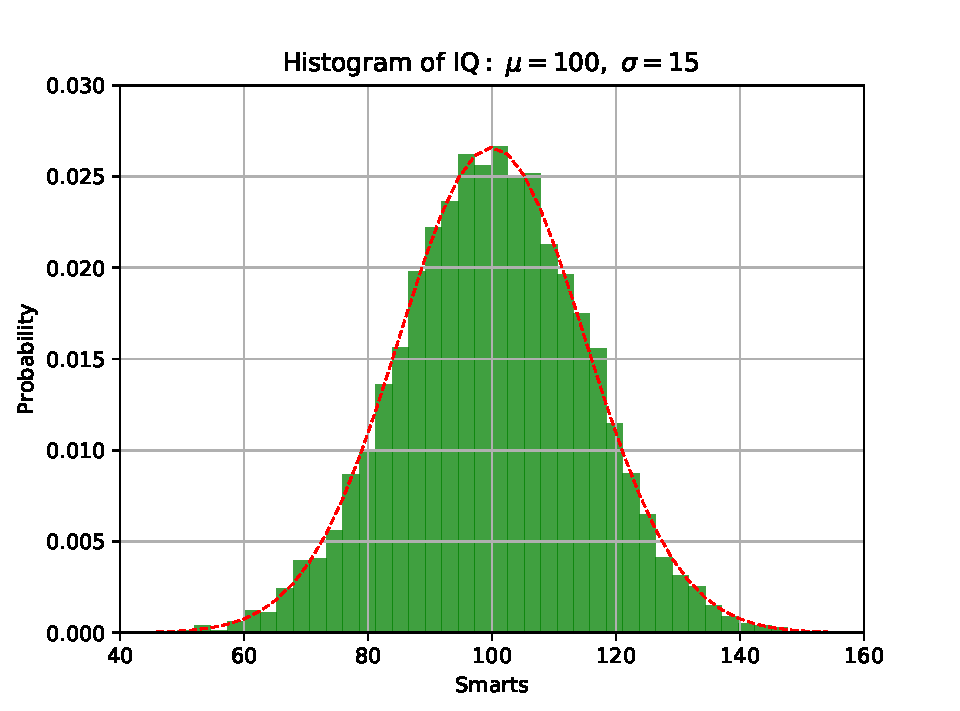
\includegraphics[width=9cm]{hist.pdf}
\end{figure}

\end{document}

